\label{buch:elliptisch:aufgabe:3}%
Aus der in Aufgabe~\ref{buch:elliptisch:aufgabe:2} konstruierten Folge
$k_n$ kann zu einem vorgegebenen $u$ ausserdem die Folge $u_n$
mit der Rekursionsformel
\[
u_{n+1} = \frac{u_n}{1+k_{n+1}}
\]
und Anfangswert $u_0=u$ konstruiert werden.
Die Landen-Transformation (siehe \cite[80]{buch:ellfun-applications})
\index{Landen-Transformation}%
führt auf die folgenden Formeln für die Jacobischen elliptischen Funktionen:
\begin{equation}
\left.\qquad
\begin{aligned}
\operatorname{sn}(u_n,k_n)
&=
\frac{
(1+k_{n+1})\operatorname{sn}(u_{n+1},k_{n+1})
}{
1 + k_{n+1} \operatorname{sn}(u_{n+1},k_{n+1})^2
}
\\
\operatorname{cn}(u_n,k_n)
&=
\frac{
\operatorname{cn}(u_{n+1},k_{n+1})
\operatorname{dn}(u_{n+1},k_{n+1})
}{
1 + k_{n+1} \operatorname{sn}(u_{n+1},k_{n+1})^2
}
\\
\operatorname{dn}(u_n,k_n)
&=
\frac{
1 - k_{n+1} \operatorname{sn}(u_{n+1},k_{n+1})^2
}{
1 + k_{n+1} \operatorname{sn}(u_{n+1},k_{n+1})^2
}
\end{aligned}
\qquad\right\}
\label{buch:elliptisch:aufgabe:3:gauss}
\end{equation}
Die Transformationsformeln
\eqref{buch:elliptisch:aufgabe:3:gauss}
sind auch als Gauss-Transformation bekannt.
\index{Gauss-Transformation}%
Konstruieren Sie daraus einen numerischen Algorithmus, mit dem sich
gleichzeitig die Werte aller drei Jacobischen elliptischen Funktionen
für vorgegebene Parameterwerte $u$ und $k$ berechnen lassen.

\begin{loesung}
In der ersten Phase des Algorithmus werden die Folgen $k_n$ und $k_n'$ 
sowie $u_n$ bis zum Folgenindex $N$ berechnet, bis $k_N\approx 0$
angenommen werden darf.
Dann gilt
\begin{align*}
\operatorname{sn}(u_N, k_N) &= \operatorname{sn}(u_N,0) = \sin u_N
\\
\operatorname{cn}(u_N, k_N) &= \operatorname{cn}(u_N,0) = \cos u_N
\\
\operatorname{dn}(u_N, k_N) &= \operatorname{dn}(u_N,0) = 1.
\end{align*}
In der zweiten Phase des Algorithmus können für absteigende
$n$ jeweils die Formeln~\eqref{buch:elliptisch:aufgabe:3:gauss}
angewendet werden um nacheinander die Werte der Jacobischen
elliptischen Funktionen für Argument $u_n$ und Parameter $k_n$
für $n=N-1,N-2,\dots,0$ zu bekommen.
\end{loesung}
\begin{table}
\centering
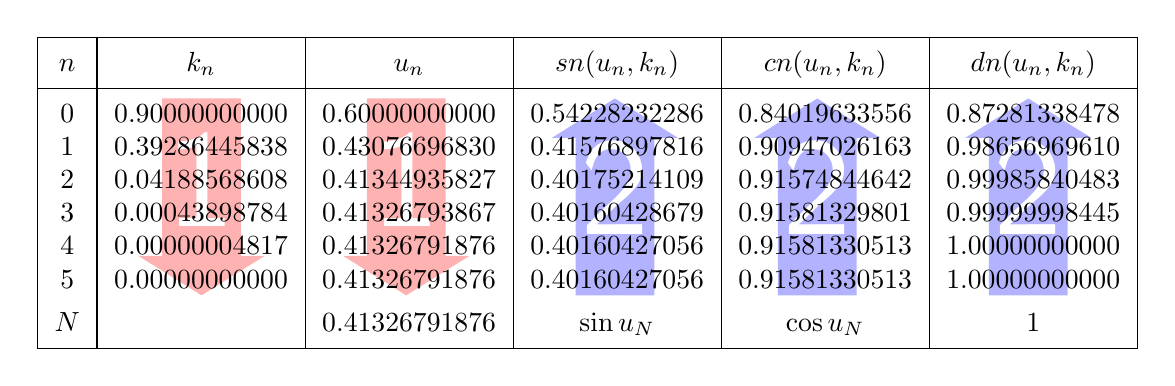
\begin{tikzpicture}[>=latex,thick]
\def\pfeil#1#2{
	\fill[color=#1!30] (-0.5,1) -- (-0.5,-1) -- (-0.8,-1)
		-- (0,-1.5) -- (0.8,-1) -- (0.5,-1) -- (0.5,1) -- cycle;
	\node[color=white] at (0,-0.2) [scale=5] {\sf #2\strut};
}
\begin{scope}[xshift=-4.9cm,yshift=0.2cm]
\pfeil{red}{1}
\end{scope}

\begin{scope}[xshift=-2.3cm,yshift=0.2cm]
\pfeil{red}{1}
\end{scope}

\begin{scope}[xshift=0.35cm,yshift=-0.3cm,yscale=-1]
\pfeil{blue}{2}
\end{scope}

\begin{scope}[xshift=2.92cm,yshift=-0.3cm,yscale=-1]
\pfeil{blue}{2}
\end{scope}

\begin{scope}[xshift=5.60cm,yshift=-0.3cm,yscale=-1]
\pfeil{blue}{2}
\end{scope}

\node at (0,0) {
\begin{tabular}{|>{$}c<{$}|>{$}c<{$}|>{$}c<{$}|>{$}c<{$}|>{$}c<{$}|>{$}c<{$}|}
\hline
n & k_n & u_n & \operatorname{sn}(u_n,k_n) & \operatorname{cn}(u_n,k_n) & \operatorname{dn}(u_n,k_n)%
\mathstrut\text{\vrule height12pt depth6pt width0pt} \\
\hline
\mathstrut\text{\vrule height12pt depth0pt width0pt}%
%\small
0 & 0.90000000000 & 0.60000000000 & 0.54228232286 & 0.84019633556 & 0.87281338478 \\
1 & 0.39286445838 & 0.43076696830 & 0.41576897816 & 0.90947026163 & 0.98656969610 \\
2 & 0.04188568608 & 0.41344935827 & 0.40175214109 & 0.91574844642 & 0.99985840483 \\
3 & 0.00043898784 & 0.41326793867 & 0.40160428679 & 0.91581329801 & 0.99999998445 \\
4 & 0.00000004817 & 0.41326791876 & 0.40160427056 & 0.91581330513 & 1.00000000000 \\
5 & 0.00000000000 & 0.41326791876 & 0.40160427056 & 0.91581330513 & 1.00000000000 \\
%N & 0.00000000000 & 0.41326791876 & 0.40160427056 & 0.91581330513 & 1.00000000000%
N &               & 0.41326791876 & \sin u_N      & \cos u_N      & 1%
%0 & 0.900000000000000 & 0.600000000000000 & 0.542282322869158 & 0.840196335569032 & 0.872813384788490 \\
%1 & 0.392864458385019 & 0.430766968306220 & 0.415768978168966 & 0.909470261631645 & 0.986569696107075 \\
%2 & 0.041885686080039 & 0.413449358275499 & 0.401752141098324 & 0.915748446421239 & 0.999858404836479 \\
%3 & 0.000438987841605 & 0.413267938675096 & 0.401604286793186 & 0.915813298019491 & 0.999999984459261 \\
%4 & 0.000000048177586 & 0.413267918764845 & 0.401604270565476 & 0.915813305135699 & 1.000000000000000 \\
%5 & 0.000000000000001 & 0.413267918764845 & 0.401604270565476 & 0.915813305135699 & 1.000000000000000 \\
%N & 0.000000000000000 & 0.413267918764845 & 0.401604270565476 & 0.915813305135699 & 1.000000000000000 \\
\mathstrut\text{\vrule height12pt depth6pt width0pt} \\
\hline
\end{tabular}
};
\end{tikzpicture}
\caption{Durchführung des auf der Landen-Transformation basierenden
Algorithmus zur Berechnung der Jacobischen elliptischen Funktionen
für $u=0.6$ und $k=0.9$.
Die erste Phase (rot) berechnet die Folgen $k_n$ und $u_n$, die zweite 
(blau)
transformiert die Wert der trigonometrischen Funktionen in die Werte
der Jacobischen elliptischen Funktionen.
\label{buch:elliptisch:aufgabe:3:resultate}}
\end{table}


